\chapter{Implementation
    \label{chapter:implementation}}

This chapter discribs the tools, methods and reasons for the from of implementation.
As sad due to early test CLIP and TinyCLIP are used as models.

\section{Model acquisition}

The CLIP models are taken from the official CLIP Github repo \cite{clipgit}.
The TinyCLIP models are taken from the official TinyCLIP Github repo \cite{tinyclipgit}.
There is also the posibility to take models from HuggingFace \cite{huggingface}.
The problem with HuggingFace is that the model cant be split into image and text encoder.
Because of this reason only models from the offical CLIP respectiv TinyCLIP repo were used.
In \cref{result:tab:clipsize} one can see the parameter count for all CLIP and TinyCLIP implementation which use a ResNet as a visual encoder.
We see that TinyCLIP uses much less parameters than the original CLIP.


\section{Model translation}
The models were first split into image and text encoder.
The image encoder then gets translated to a onnx graph and afterwards simplified.
This onnx graph then is translated by the \acrshort{dfc} to \acrshort{har} and \acrshort{hef} files.

\begin{figure}
    \centering
    \subfloat[End of CLIP ResNet50x4 vision encoder Onnx graph acquired though official CLIP]{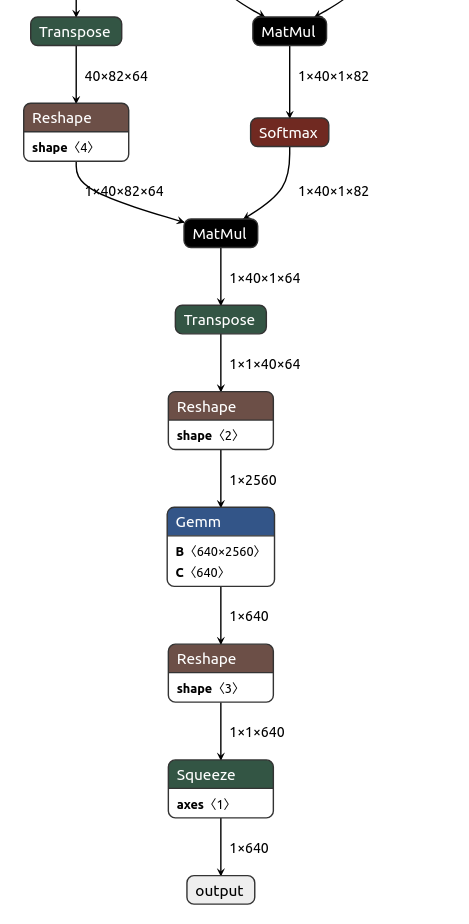
\includegraphics[width=0.4\textwidth]{Images/Implementation/ClipRes50x4.png}\label{fig:implementation:clipres50x4}}
    \qquad
    \subfloat[End of CLIP ResNet 50x4 vision encoder Onnx graph sendt by Hailo]{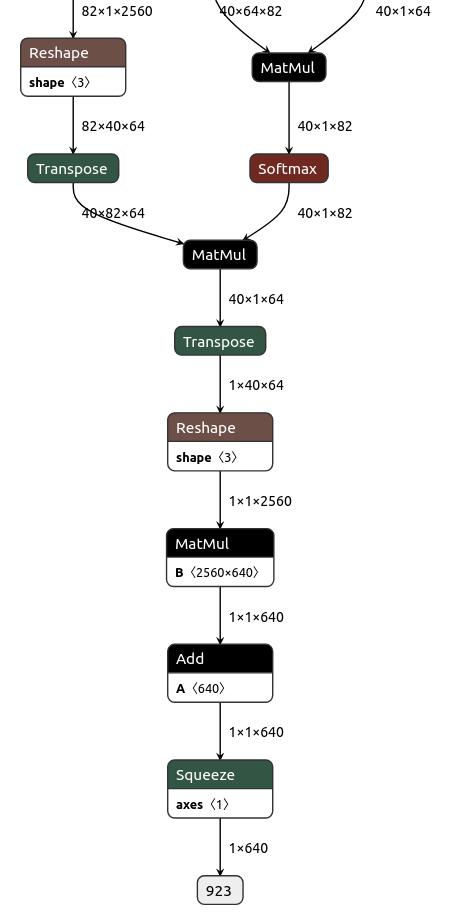
\includegraphics[width=0.4\textwidth]{Images/Implementation/HailoClipRes50x4.png}\label{fig:implementation:hailoclipres50x4}}
    \caption{Comparison of CLIP ResNet 50x4 vision encoder Onnx graph (a) from official CLIP and (b) from Hailo. The important thing to see are the numbers of dimensions.}
    \label{fig:implementation:compareRN50x4}
\end{figure}

In that step lays the first big problem of the project.
As described in \cref{section:dfc} the \acrshort{dfc} is unable to compile transformers.
To be precise, a transpose block at the end of every self attention layer is were the problems lay.
The \acrshort{dfc} swaps dimensions and takes together the last 2 dimensions.
In the ResNet which is acquired through the offical code (see \cref{fig:implementation:clipres50x4}) one can see that the transpose block after the MatMul block swaps a second and the third dimension.
This leads to a compilation error because the \acrshort{dfc} already combined the last 2 dimensions.
This error does not occure when the model given by Hailo is compiled.
This is becaues the networks from hailo are acquired with a older version of CLIP and the ONNX exporter.
The graph are functionaly the same but are diffrent in architecture.
In \cref{fig:implementation:hailoclipres50x4} the maximum of dimensions of the network from Hailo is 3.

To work around this problem the last part of the onnx graph is cut off.
To cut the graph Onnx-Modifier \cite{onnxmodifier} is used.
The cut off blocks are implemented as postprocessing.
As described in \cref{section:dfc} a script can be applied to change the behavior of the \acrshort{dfc}.
% Add scripts

After quantisation the graph can again be visualized with a tool name profiler from hailo.
In \cref{fig:implementation:compareRN50x4qunathar} the compiled model with the cutoff end is visualized.
In this figure the combination of the last dimensions can be seen.

\begin{figure}
    \centering
    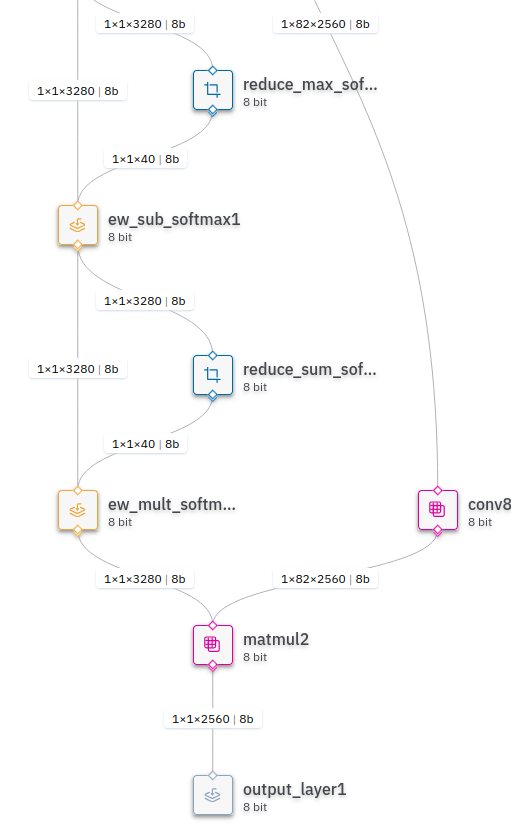
\includegraphics[width=0.4\textwidth]{Images/Implementation/ClipRes50x4_qunat_Har.png}
    \caption{Output of the \acrshort{dfc} from compiling the modified onnx graph of the ResNet50x4.}
    \label{fig:implementation:compareRN50x4qunathar}
\end{figure}

This graph then gets compiled to a \acrshort{hef} file which can be executed on Hailo hardware.
To use CLIP the text embeddings are also needed.
Due to the limitation that no transformers can be used with hailo the embeddings get calculated on a PC and the saved in a Json file.

\subsection{Pre-processing}

The hexagon dataset which is used as refrence consists of panorama pictures.
These pictures get cut into 5 equal sized patches.
Every patch gets processed with CLIP.
To process one of these patches with CLIP they have to be preprocessed by resizing them to the specific input size.
The preprocess consits of the following steps:
\begin{itemize}
    \item Resize
    \item Centercrop
    \item If not already RGB transform image to RGB
    \item Normalize
\end{itemize}
Normalization values are calculate over the whole Hexagon dataset.
Finally a mayority vote is taken over the subclasses of the patches to classify a image.
This process is mentiond in Lia Winkler's report and increases the accuracy of the predictions.

\subsection{Post-processing}

As sad the cut of part of the Onnx graph is processed in post processing.
The Cut of part consists of one matrix multipication and some rearanging of the dimensions.
In a first implementation the weights for the matrix multipication were extracted and saved in a json file.
In a second attemp the cut off Onnx Graph is directly used.
The second attemp proved faster while using less memory.


\section{Inference}

To have a good comparison of performance the implementation on the Raspberry Pi is mostly similar to the one which is used on PC.
The PC application is mostly the same as Lia Winkler used in her work.
For Vision encoder only ResNet's were used because of the limitations from the \acrshort{dfc}.
The Hexagon dataset is used as image input.
As text input the subclasses from \cref{tab:dataset:subclasses} are used.
The text input are used in scentens.
In \cite{clip} the authors state that the performance of the network can improve if the text inputs are in a scentens.
To use the vision model on Hailo the python api is used.
2 diffrent implmentations were tested.
The first implementation is based on a code snippet found on \cite{hailoimplementation}.
In this implementation initialises the device every time a output is calculated.
This makes the programm very slow and no significant speed up is achieved.

The second implementation corrects this problem.
The device gets initialised once at the start of the programm.
With this approach a speed up of the factor 2 can be achieved in comparison to the evaluation on the PC CPU



The accuracy reduces significant after quantisation. 

\section{Evaluation}

To measure the performance of the Hailo hardware the models were tested in 3 ways:
\begin{itemize}
    \item CPU PC
    \item CPU Raspberry Pi
    \item Hailo hardware accelerator
\end{itemize}
The implementations were made as similiar as possible to ensuer the values are correct and representiv. 
As values to measure the following found usefull:
\begin{itemize}
    \item Throughput(speed)
    \item Accuracy
    \item Mermory(parameter count and size) 
\end{itemize}

For throughput 2 measurments are taken.
The first measures the time from input to output.
This includes calculating the text embeddings, the image embeddings and the dot product of the embeddings.
This measurment is called throughput and is measured in iterations per second (it/s).
The second measures the time it takes to calculate one image embedding.
This measurment is called throughput image and is also measured in iterations per second (it/s).

The accuracy of a model describes how a model performs in labeling pictures as in- or outdoor.
This measurment is taken because it is an easy way to see if a network is working correct but it can easly give a wrong image of the situation because it doesnt take unbalanced datasets in consideration.
To get a precise answer if the network is working correct the confusion matix or a class report of a model has to evaluated.
Both of these are found in the appendix.

The models get executed on the edge.
Although a Raspberry Pi has plenty of mermory it is always a good practice to include the size of a model as measurment.
Size is measured in memory or parameter count.

\subsection{Without hardware accelerator}
In \cref{methods:tab:perfPC} the performance on a PC CPU is displayed.
These values 
These values are used to compare the performance with the hailo hardware accelerator.

\begin{table}[]
    \centering
    \begin{tabular}{l|rrrrr}
    \hline
        Modelname & Accuracy & \makecell{Throughput\\(it/s)} & \makecell{Throughput \\ Image (it/s)} & Throughput std & \makecell{Throughput\\Image std} \\ \hline
        RN50 & 0.982 & 12.46 & 32.48 & 5.33 & 3.18 \\ 
        RN101 & 0.984 & 9.38 & 20.01 & 3.43 & 1.81 \\ 
        RN50x4 & 0.989 & 5.79 & 12.13 & 2.04 & 0.86 \\ 
        RN50x16 & 0.963 & 2.51 & 3.81 & 0.55 & 0.17 \\ 
        RN50x64 & 0.988 & 0.88 & 1.13 & 0.11 & 0.03 \\ 
        TinyCLIP-19M & 0.985 & 20.38 & 54.06 & 8.37 & 3.65 \\ 
        TinyCLIP-30M & 0.988 & 13.59 & 37.53 & 5.72 & 3.31 \\ 
    \end{tabular}
    \caption{Performance table from evalutaion on PC CPU.}
    \label{methods:tab:perfPC}
\end{table}

In \cref{methods:tab:perfRaspi} the performance measurments from executing on the Raspberry Pi CPU are displayed.
RN50x16 and RN50x64 are missing because they are too big to evaluate.
As one can expect the throughput on the Raspberry Pi is significant lower than the throughput on the PC CPU from \cref{methods:tab:perfPC} because of the lower computing power.
Intresting is that the accurcy from \cref{methods:tab:perfRaspi} is slightly different to \cref{methods:tab:perfPC}.
This can be explaind by diffrent CPU architectures and some floating point rounding.
In \cref{methods:tab:perfRaspi} the parameter count of the image encoder is displayed. These values are the same for the models on PC and Raspberry Pi.

\begin{table}[]
    \centering
    \begin{tabular}{l|rrrrr}
    \hline
    Modelname & Accuracy & \makecell{Throughput\\(it/s)} & \makecell{Throughput \\ Image (it/s)} & Throughput std & \makecell{Throughput\\Image std} \\ \hline
        RN50 & 0.979 & 1.15 & 2.85 & 0.36 & 0.05 \\ 
        RN101 & 0.982 & 0.92 & 1.89 & 0.24 & 0.038 \\ 
        RN50x4 & 0.988 & 0.61 & 1.13 & 0.14 & 0.0162 \\ 
        TinyCLIP-19M & 0.982 & 2.27 & 5.22 & 0.63 & 0.16 \\ 
        TinyCLIP-30M & 0.983 & 1.60 & 3.79 & 0.47 & 0.09 \\ 
    \end{tabular}
    \caption{Performance table from evalutaion on Raspberry Pi CPU.}
    \label{methods:tab:perfRaspi}
\end{table}

\begin{table}[]
    \centering
    \begin{tabular}{l|rr}
    \hline
    Model name & \begin{tabular}[c]{@{}l@{}}Parameters\\ Visual(Mio)\end{tabular} & \begin{tabular}[c]{@{}l@{}}Parameters\\ Text(Mio)\end{tabular} \\ \hline
    RN50                & 38.3  & 37.8  \\
    RN50x4              & 87.1  & 59.1  \\
    RN50x16             & 167.3 & 850.5 \\
    RN50x64             & 420.4 & 151.1 \\
    RN101               & 56.3  & 37.8  \\
    TinyCLIP-19M & 18.5  & 18.9  \\
    TinyCLIP-30M & 29.5  & 28.3  \\ 
    \end{tabular}
    \caption{Paramter count for different CLIP implementations with ResNet as visual encoder}
    \label{methods:tab:clipsize}
\end{table}



\subsection{With hardware accelerator}
\begin{table}[]
    \centering
    \begin{tabular}{l|rr}
    \hline
    Model name & \begin{tabular}[c]{@{}l@{}}Parameters\\ Visual(Mio)\end{tabular} \\ \hline
    RN50                & 36.2  \\
    RN50x4              & 85.3  \\
    RN50x16             & 164.6 \\
    RN101               & 55.1 \\
    TinyCLIP-19M & 17.1  \\
    TinyCLIP-30M & 27.7  \\ 
    \end{tabular}
    \caption{Paramter count for different CLIP implementations with ResNet as visual encoder}
    \label{methods:tab:clipsizequant}
\end{table}

Now networks after compilation are examined.
First we take a look on the paramter count.
There is a slight decrease in paramters but this can be explaind.
In the case of TinyCLIP-19M the cut off graph consists of a matrix multipication with a matrix of the shape \(1024 \times 1408\).
With 
\begin{equation*}
    1024 \times 1408 + 1024 = 1'442'816
\end{equation*}
we get the parameter count for the cut off graph.
Now this gets added to the paramter count of the model and this results in 
\begin{equation*}
    1.4 \text{M} + 17.1 \text{M} = 18.5 \text{M} 
\end{equation*}
which is the parameter count before compilation(see \cref{methods:tab:clipsize}).
This calculation can also be done for all other models but the result is the same.
This result means that the architecture isnt affected by the \acrshort{dfc}.
It only changes the quantisation.
Because of quantisation the mermory size should be around 4 times lower than before because the datatype which changes from FP32 to INT8.
This assumtion cant be verfied because the datatype from before and after arent the same.

\begin{table}[!h]
    \centering
    \begin{tabular}{l|rrrrr}
    \hline
    Modelname & Accuracy & \makecell{Throughput\\(it/s)} & \makecell{Throughput \\ Image (it/s)} & Throughput std & \makecell{Throughput\\Image std} \\ \hline
    RN50 & 0.983 & 20.63 & 24.58 & 1.341 & 0.27 \\ 
    RN50x4 & 0.982 & 10.13 & 10.75 & 0.32 & 0.059 \\ 
    RN101 & 0.981 & 15.61 & 17.09 & 0.49 & 0.081 \\
    TinyClip19M & 0.017 & 30.41 & 39.29 & 2.71 & 3.02 \\ 
    TinyClip30M & 0.530 & 22.96 & 27.82 & 1.57 & 1.71 \\ 
    \end{tabular}
    \label{methods:tab:perfHailo}
    \caption{Performance table from evalutaion on Hailo 8L.}
\end{table}

Now lets take a look at speed and accuracy.
In \cref{methods:tab:perfHailo} the performance table for hailo is displayed.
First we see that the throughput is much higher compared to the performance on the Raspberry Pi CPU (see \cref{methods:tab:perfRaspi}).
On the first look the accuracy only dropped when using TinyCLIP models.
But the accuracy of the other ResNet's also paints a wrong picture.
To see the real situation one has to look at the confusion matrix of RN50 (see \cref{methods:fig:compareConfM}).
There we see that although the accuracy is fine many pictures get misclassified.

\begin{figure}[!h]
    \centering
    \subfloat[][Evaluation on PC]{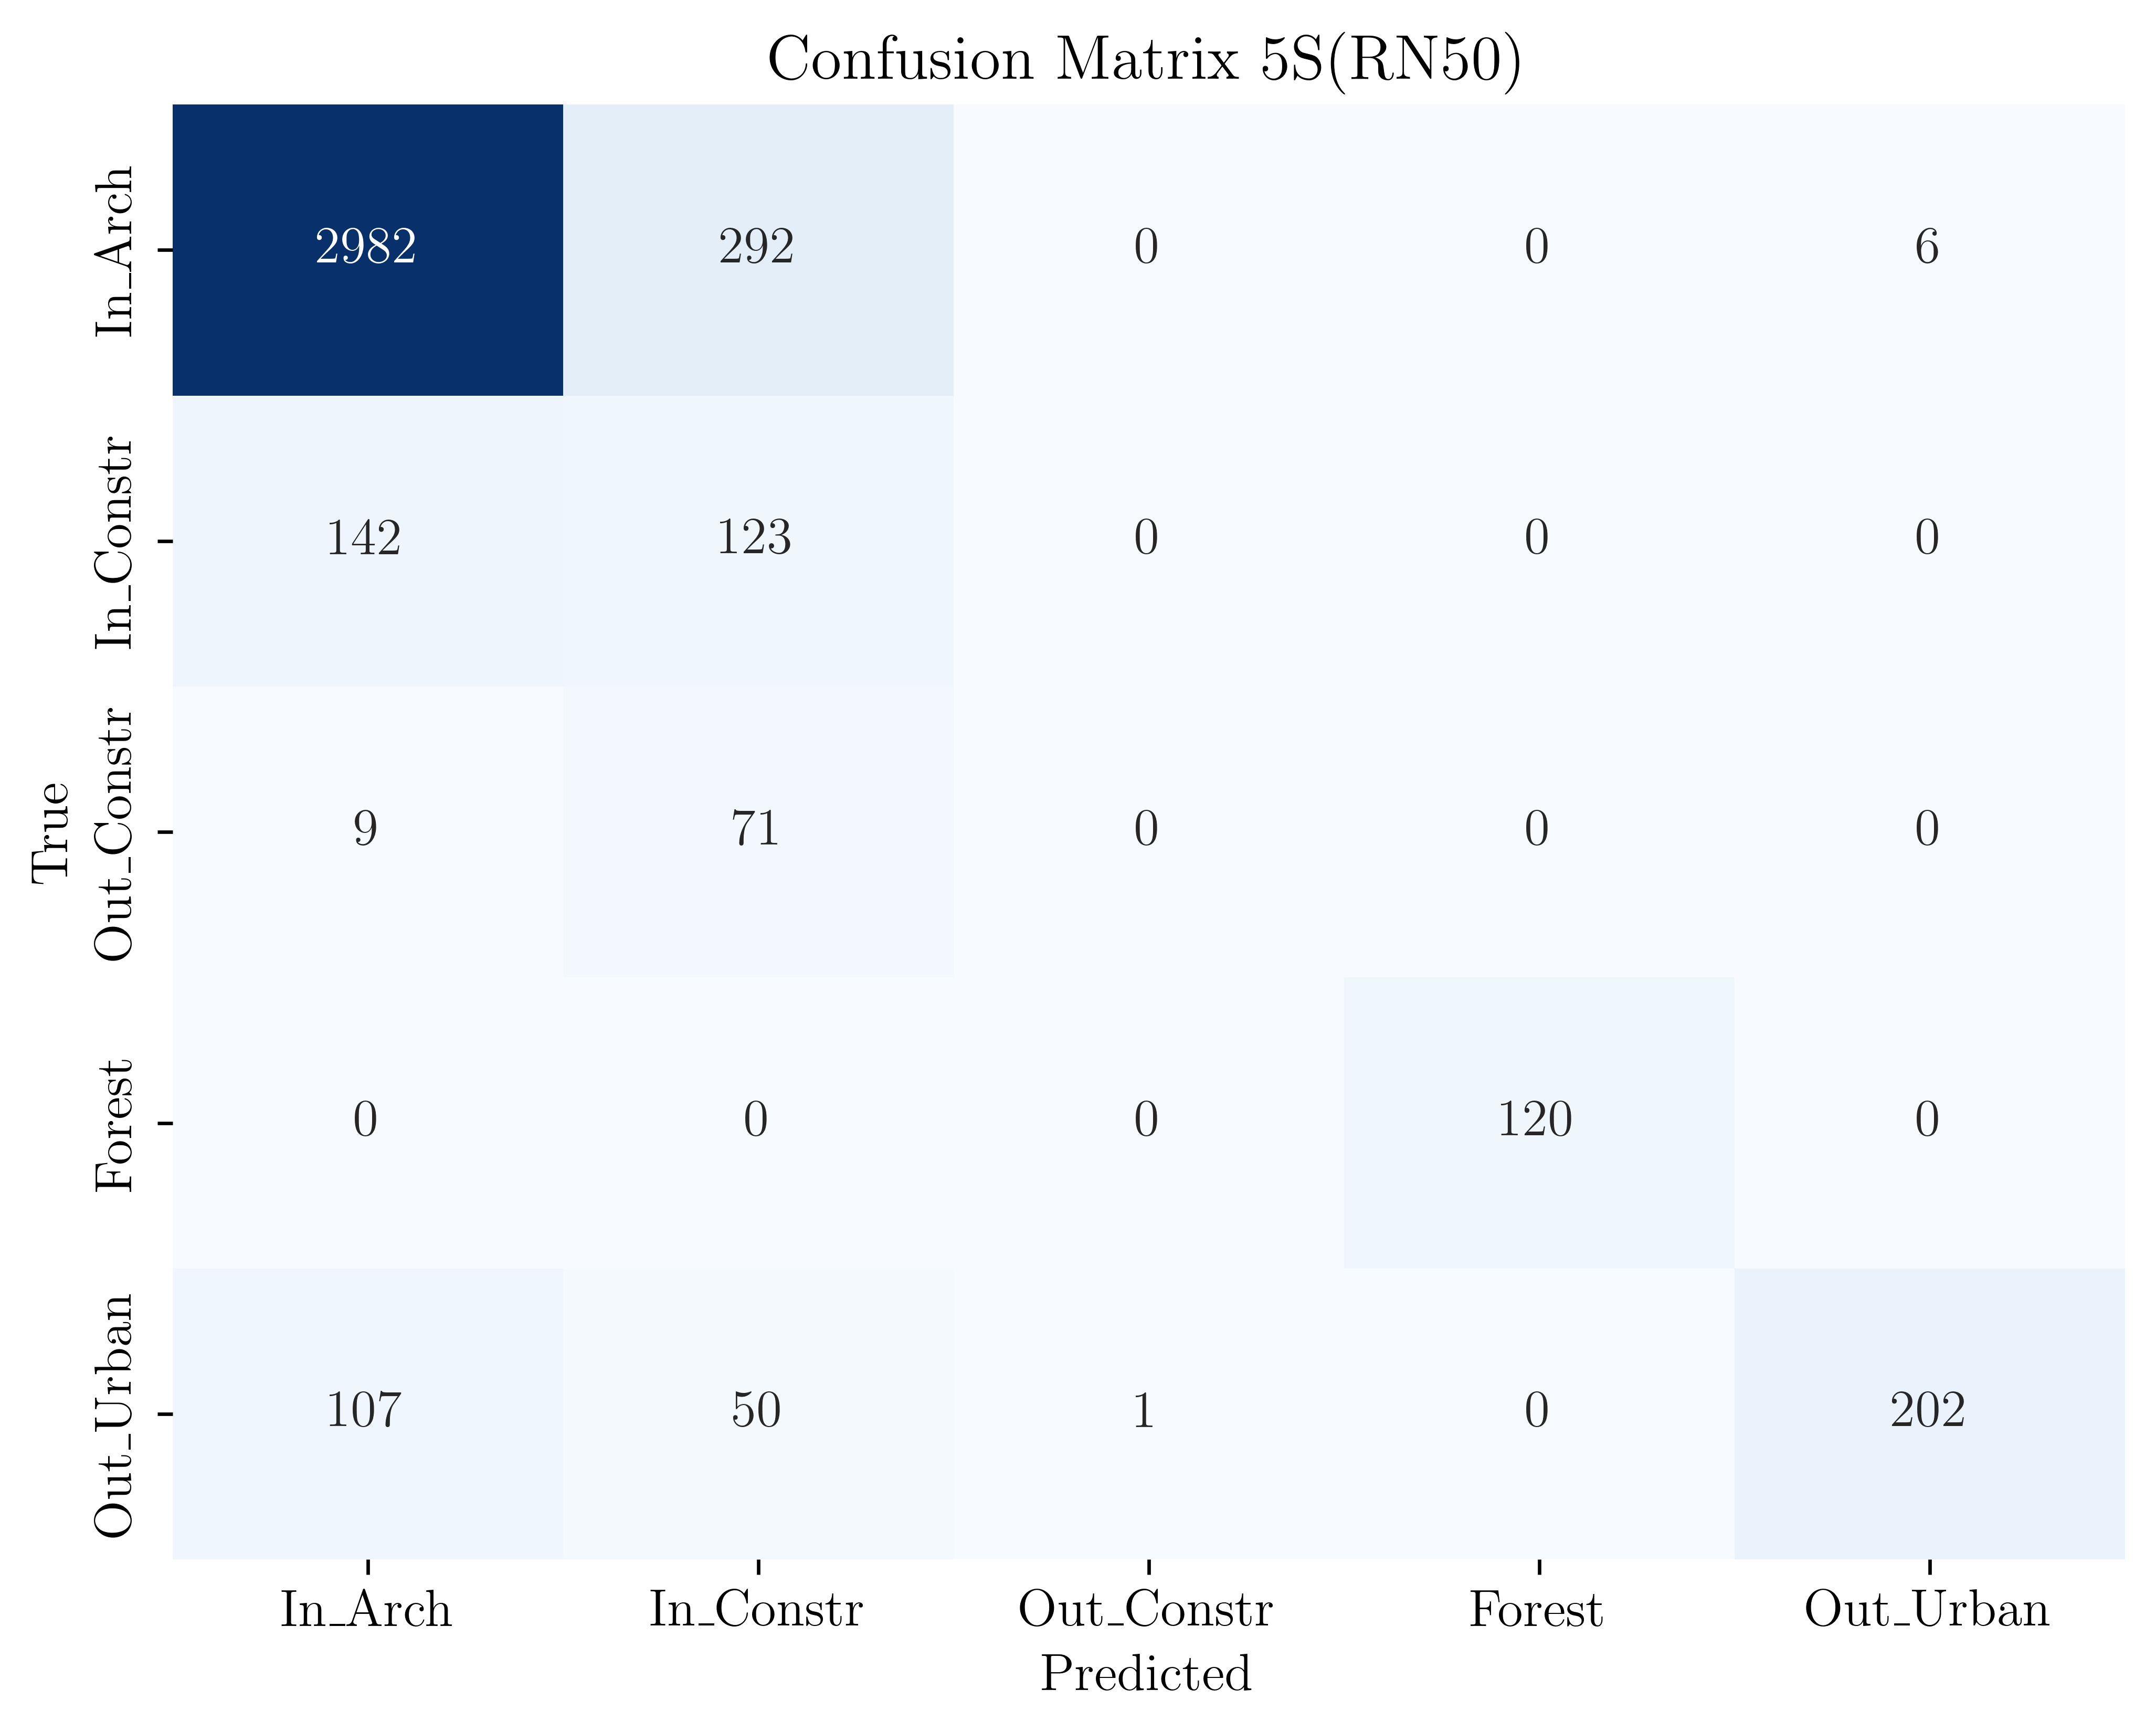
\includegraphics[width=0.49\textwidth]{Images/appendix/resultsPC/Confusion Matrix 5S(RN50).png}\label{methods:fig:confrn50pc}}
    \subfloat[][Evaluation on Hailo]{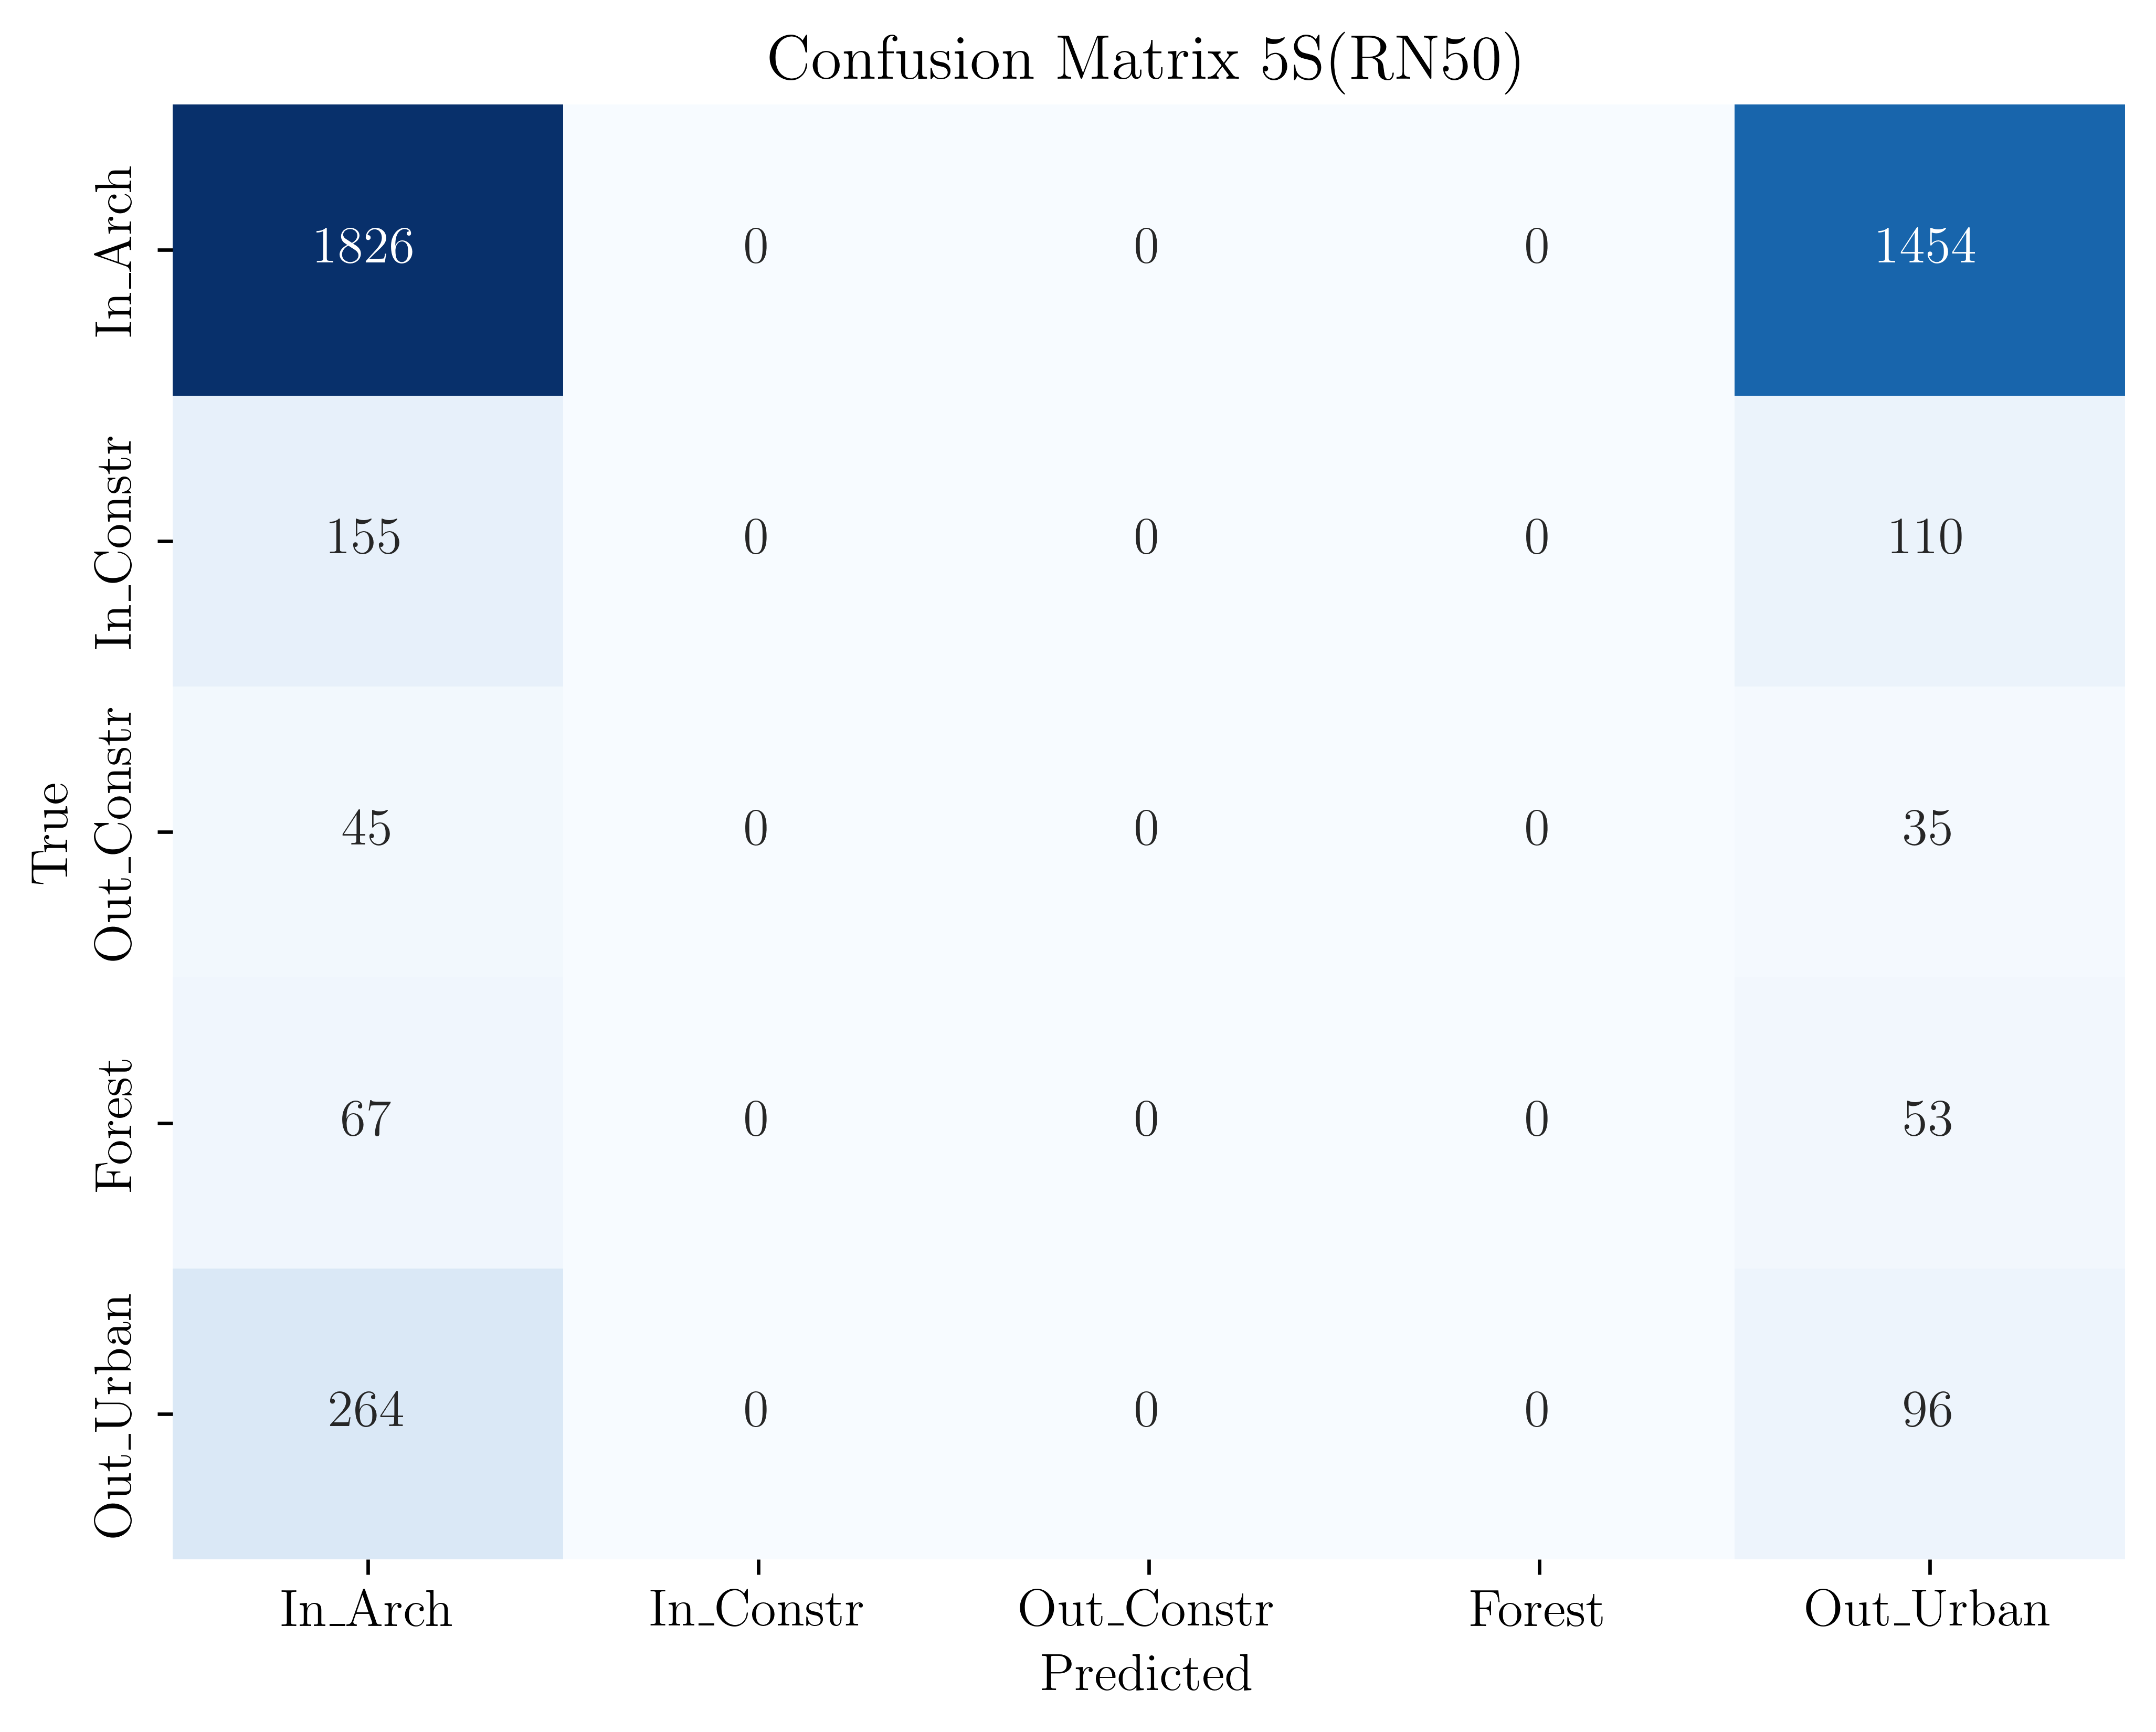
\includegraphics[width=0.49\textwidth]{Images/Implementation/Confusion Matrix 5S(RN50)Hailo.png}\label{methods:fig:confrn50hailo}}
    \label{methods:fig:compareConfM}
    \caption{Comparison of confusion matrix from Hailo to PC}
\end{figure}

There are a couple reasons for that:
\begin{itemize}
    \item There is an error in the implementation. This could be in the creation of the confusion matrix or in postprocessing.
    \item The text embeddings are different.
    \item Because of bad quantisation the model cant classify the pictures correct.
\end{itemize}

\section{Controll Implementation
    \label{scetion:methods:contimp}}
First and easy to check is the creation of the confusion matrix because the same code is used on Hailo and on PC.

Second the text embeddings.
As menationd earlier the text embeddings are safed in an json file.
Possible erros could be that the embeddings are safed wrong or by that converting the values also rounds them.
To check for these errors the differents between the output of text encoder and the json file is taken.
In all cases the differents is zero.
This means that the values are identical.

\begin{figure}[h]
    \centering
    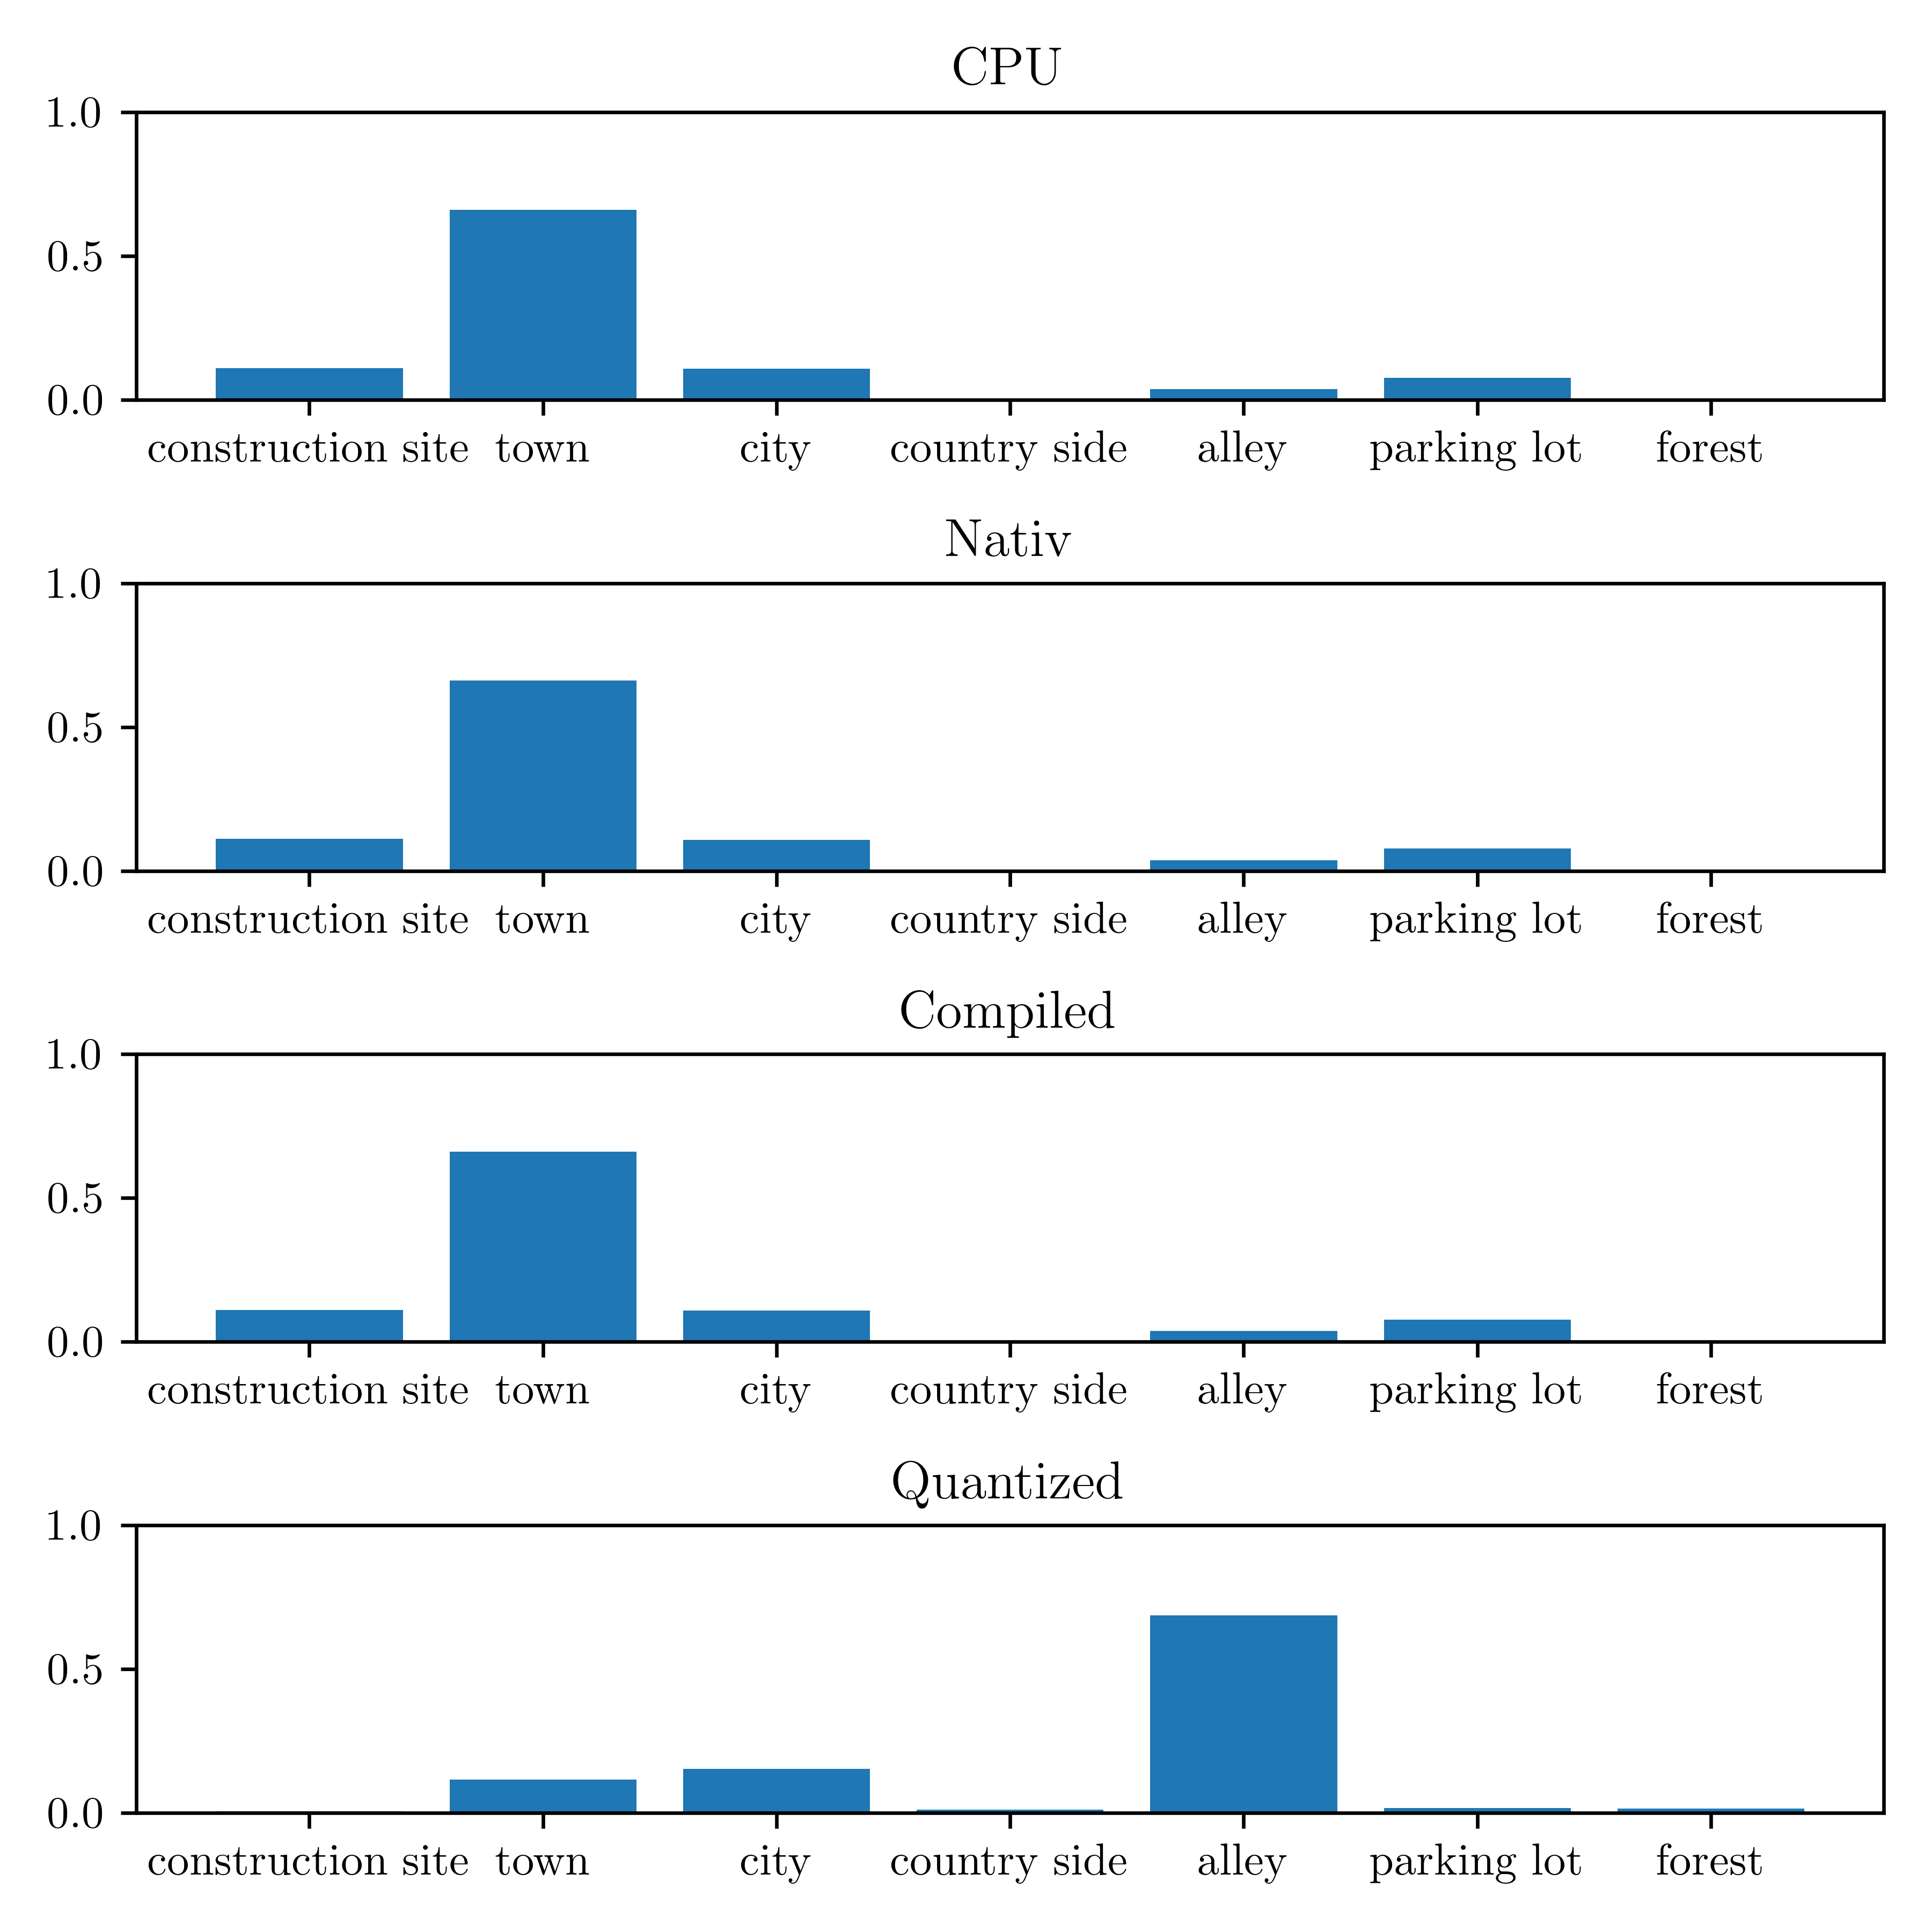
\includegraphics[width=0.6\textwidth]{Images/Implementation/compareProbs_RN50.png}
    \caption{Compare outputs at different \acrshort{dfc} points with RN50.}
    \label{methods:fig:comparern50}
\end{figure}

To check the functionality, the output and of the quantisation the output of the \acrshort{dfc} is checked at every stage.
The \acrshort{dfc} is able to calculate the output of the compiling network at every step.
With that the postprocessing and the functionality of the quantisation can be checked.
The test is conducted with a test image (see \cref{methods:fig:comparetestpic}).
The Results can be seen in \cref{methods:fig:comparern50}.
First we see that the output from CPU, Nativ and Compiled are the same.
This confirms that postprocessing is implemented correct.
We see that after quantisation there is a huge shift of the output.
The effect can also be seen on the output of other images.
This indicates that the quantisation is the problem.

\begin{figure}
    \centering
    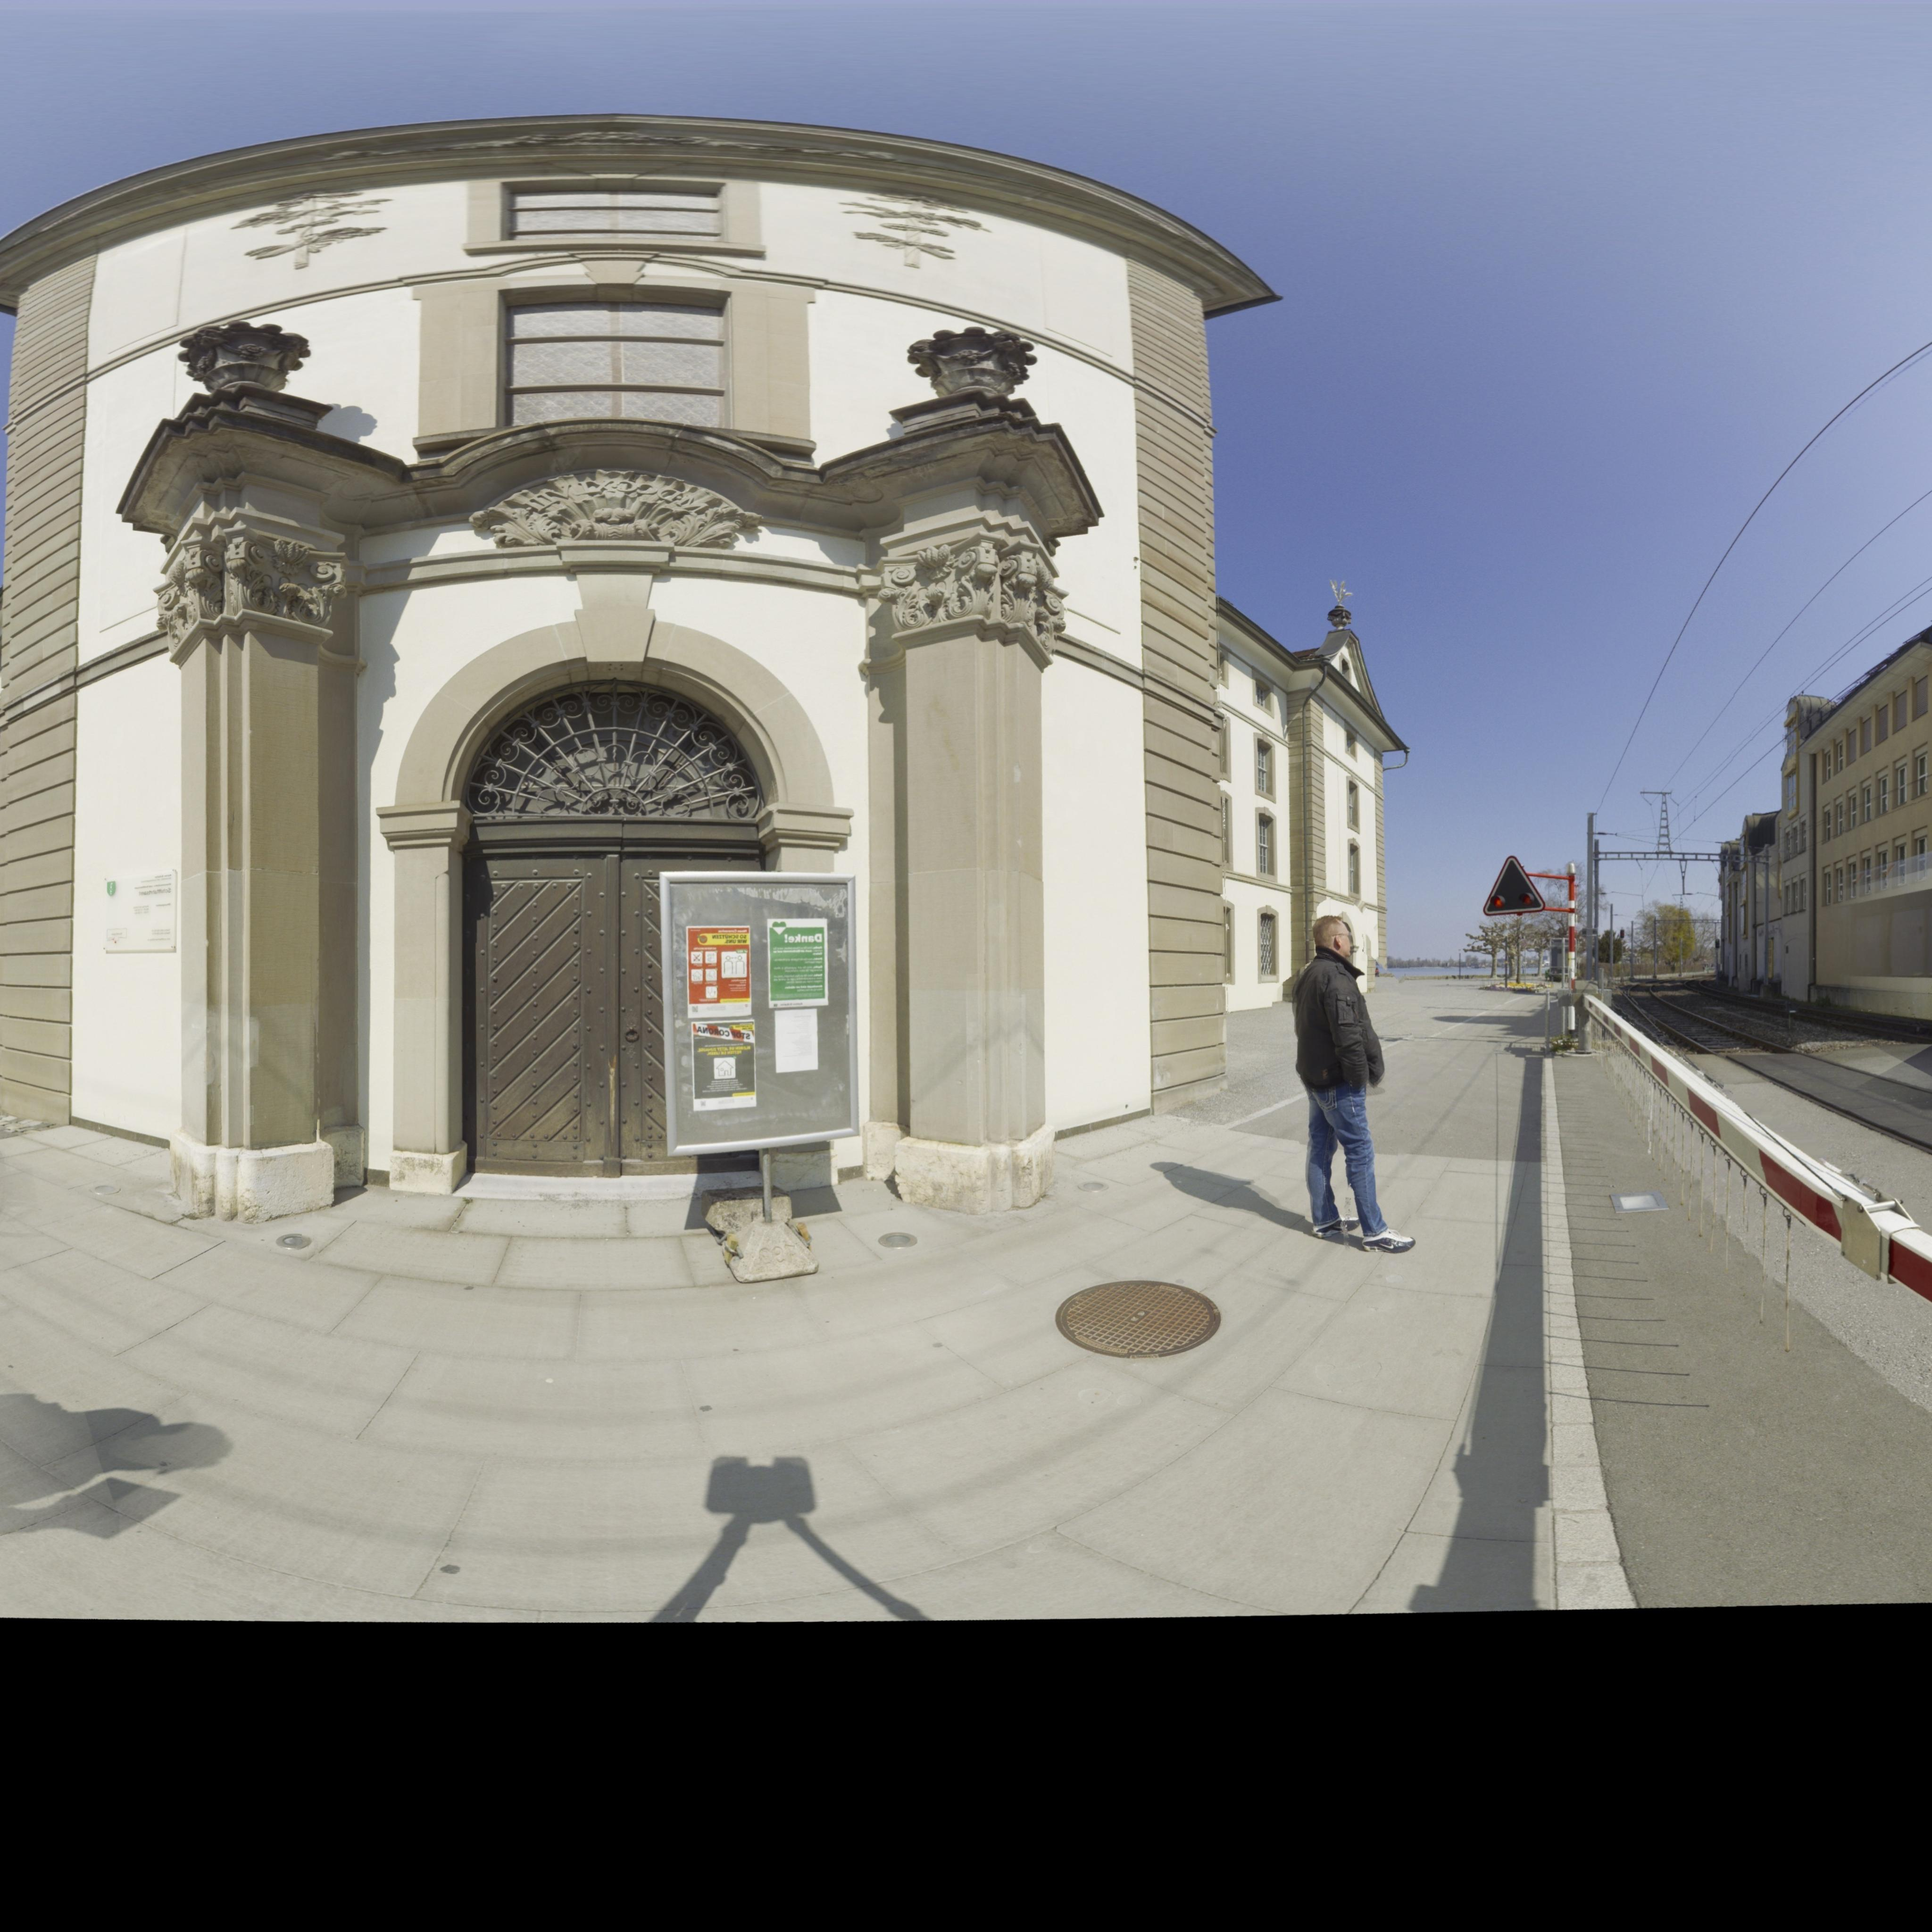
\includegraphics[width=0.5\textwidth]{Images/Implementation/panorama_00002_0014_2_testIMg.jpg}
    \caption{Testimage [panorama\_00002\_0014\_2] to compare outputs of the \acrshort{dfc}}
    \label{methods:fig:comparetestpic}
\end{figure}

\section{Increase accuracy}

In \cref{scetion:methods:contimp} the reason for the bad accuracy is suspected to be the bad quantisation.
The models are all translated to INT8.
In a attemp to increase accuracy as much as possible is convertet to INT16.
Other ways to increase the accuracy are better text promts and adjusting the threshold for binary classifications.


\subsection{Change quantisation}

The \acrshort{dfc} offers a way to change the quantisation of the weigths.
This is applied via the model script in quantisation.


\subsection{Adjust threshold}

A way to increase accuracy is to adjust the threshold.
This only works in binary classification.
This can be applied to the classification between indoor and outdoor and indoor construction and architectural.
For the outdoor classes (forest,urban and out construction) nothing like this can be done to increase the accuracy.
This threshold has to be calculate.
For this calculation one has to watch out to use a balanced dataset.
To get a balanced dataset a subset is created so that each class has the same amount of images.
The images are randomly sampled.

\subsection{Change cut location}
Most of the examples from the hailo model zoo\cite{hailo_model_zoo} are CNN's.
A assumption is that the last part of the ResNet's a self attention layer isnt quantising propely due to some big matrix multipications.

To work against this effect the cut which in any case has to be made can appear earlier in the graph.
This leads to a lower throughput but may increase the accuracy.